\documentclass{article}
\usepackage[landscape]{geometry}
\usepackage{url}
\usepackage{multicol}
\usepackage{amsmath}
\usepackage{esint}
\usepackage{amsfonts}
\usepackage{tikz}
\usetikzlibrary{decorations.pathmorphing}
\usepackage{amsmath,amssymb}
\usepackage{listings}
\usepackage{colortbl}
\usepackage{xcolor}
\usepackage{mathtools}
\usepackage{amsmath,amssymb}
\usepackage{enumitem}
\usepackage{environ}
\usetikzlibrary{shapes,snakes}

\makeatletter

\newcommand*\bigcdot{\mathpalette\bigcdot@{.5}}
\newcommand*\bigcdot@[2]{\mathbin{\vcenter{\hbox{\scalebox{#2}{$\m@th#1\bullet$}}}}}
\makeatother

\title{}
\usepackage[brazilian]{babel}
\usepackage[utf8]{inputenc}

\advance\topmargin-.8in
\advance\textheight3in
\advance\textwidth3in
\advance\oddsidemargin-1.5in
\advance\evensidemargin-1.5in
\parindent0pt
\parskip2pt
\newcommand{\hr}{\centerline{\rule{3.5in}{1pt}}}
%\colorbox[HTML]{e4e4e4}{\makebox[\textwidth-2\fboxsep][l]{texto}


\definecolor{blue}{HTML}{A7BED3}
\definecolor{brown}{HTML}{DAB894}
\definecolor{pink}{HTML}{FFCAAF}


\DeclareMathOperator{\Unif}{Unif}
\DeclareMathOperator{\Var}{Var}
\DeclareMathOperator{\Cov}{Cov}
\DeclareMathOperator{\Bern}{Bernoulli}
\DeclareMathOperator{\Bin}{Bin}
\DeclareMathOperator{\Pois}{Poisson}
\DeclareMathOperator{\atanh}{arctanh}


\DeclareMathOperator{\vif}{VIF}
\DeclareMathOperator{\aic}{AIC}
\DeclareMathOperator{\bic}{BIC}
\DeclareMathOperator{\sch}{Sch}
\DeclareMathOperator{\bias}{Bias}
\DeclareMathOperator{\press}{PRESS}
\DeclareMathOperator{\fin}{IN}
\DeclareMathOperator{\fout}{OUT}

\DeclareMathOperator{\odds}{odds}
\DeclareMathOperator{\diag}{diag}
\DeclareMathOperator{\dev}{Dev}
\DeclareMathOperator{\length}{length}




\newtheorem{theorem}{Theorem}[section]
\newtheorem{definition}{Definition}[section]
\newtheorem{fact}{Fact}[section]
\newtheorem{prop}{Proposition}[section]
\newtheorem{corollary}{Corollary}[section]





\tikzset{header/.style={path picture={
\fill[green, even odd rule, rounded corners]
(path picture bounding box.south west) rectangle (path picture bounding box.north east) 
([shift={( 2pt, 4pt)}] path picture bounding box.south west) -- 
([shift={( 2pt,-2pt)}] path picture bounding box.north west) -- 
([shift={(-2pt,-4pt)}] path picture bounding box.north east) -- 
([shift={(-6pt, 6pt)}] path picture bounding box.south east) -- cycle;
},
label={[anchor=west, fill=green]north west:\textbf{#1:}},
}} 

\tikzstyle{mybox} = [draw=black, fill=white, very thick,
    rectangle, rounded corners, inner sep=10pt, inner ysep=10pt]
\tikzstyle{fancytitle} =[fill=black, text=white, rounded corners, font=\bfseries]


\tikzstyle{bluebox} = [draw=blue, fill=white, very thick,
    rectangle, rounded corners, inner sep=10pt, inner ysep=10pt]
\tikzstyle{bluetitle} =[fill=blue, inner sep=4pt, text=white, font=\small]


\tikzstyle{brownbox} = [draw=brown, fill=white, very thick,
    rectangle, rounded corners, inner sep=10pt, inner ysep=10pt]
\tikzstyle{browntitle} =[fill=brown, inner sep=4pt, text=white, font=\small]

\tikzstyle{pinkbox} = [draw=pink, fill=white, very thick,
    rectangle, rounded corners, inner sep=10pt, inner ysep=10pt]
\tikzstyle{pinktitle} =[fill=pink, inner sep=4pt, text=white, font=\small]

\tikzstyle{redbox} = [draw=red!35, fill=white, very thick,
    rectangle, rounded corners, inner sep=10pt, inner ysep=10pt]
\tikzstyle{redtitle} =[fill=red!35, inner sep=4pt, text=white, font=\small]


\NewEnviron{brownbox}[1]{
    \begin{tikzpicture}
    \node[brownbox](box){%
    \begin{minipage}{0.9\textwidth}
    \BODY
    \end{minipage}};
    \node[browntitle, right=10pt] at (box.north west) {#1};
    \end{tikzpicture}
}

 \NewEnviron{redbox}[1]{
    \begin{tikzpicture}
    \node[redbox](box){%
    \begin{minipage}{0.9\textwidth}
    \BODY
    \end{minipage}};
    \node[redtitle, right=10pt] at (box.north west) {#1};
    \end{tikzpicture}
}
   
    

\NewEnviron{bluebox}[1]{%
\begin{tikzpicture}
    \node[bluebox](box){%
        \begin{minipage}{0.9\textwidth}
            \BODY
        \end{minipage}
    };
    
\node[bluetitle, right=10pt] at (box.north west) {#1};
\end{tikzpicture}
}

\NewEnviron{pinkbox}[1]{%
\begin{tikzpicture}
    \node[pinkbox](box){%
        \begin{minipage}{0.9\textwidth}
            \BODY
        \end{minipage}
    };
    
\node[pinktitle, right=10pt] at (box.north west) {#1};
\end{tikzpicture}
}



\NewEnviron{blackbox}[1]{%
\begin{tikzpicture}
    \node[mybox](box){%
        \begin{minipage}{0.3\textwidth}
        \raggedright
        \small{
            \BODY
        }
        \end{minipage}
    };
    
\node[fancytitle, right=10pt] at (box.north west) {#1};
\end{tikzpicture}
}


\begin{document}

\begin{center}{\large{\textbf{Formal Languages Summary}}}\\
\end{center}




\begin{multicols*}{3}

\begin{blackbox}{Defining Languages}
    \textbf{Definition.} An \emph{alphabet} is a finite set of symbols.\\
    \textbf{Definition.} A \emph{language} is defined as a set of exhaustive list of words or set of rules defining accepted words over an alphabet.\\
    \textbf{Definition.} A \emph{word} or \emph{string} is a sequence of symbols from an alphabet.\\
    \textbf{Definition.} The \emph{length} of a string is the number of letters in a string, is 0 when string is empty ($\Lambda$).
    \textbf{Theorem 1.} For any set of strings $S$, we have $S^* = S^{**}$.
\end{blackbox}
\begin{blackbox}{Recursive Definitions}
    A \emph{recursive definition} is a 3 part definition:
    \begin{enumerate}[leftmargin=0.5cm]
        \item First, specificy some basic objects in the set.
        \item Second, give rules for constructing new objects from the basic ones.
        \item Third, specify that no objects are in the set unless they are constructed in this way.
    \end{enumerate}
    \begin{bluebox}{Theorems}
        \textbf{Theorem 2.} An arithmetic expression cannot contain the character \$.\\
        \textbf{Theorem 3.} No arithmetic expression can begin or end with the symbol /.\\
        \textbf{Theorem 4.} No arithmetic expression can contian the substring //.
    \end{bluebox}
    \textbf{Propositional Calculus.} The set of all well-formed formulas (wffs) defined on the alphabet \\[-1ex]
    \[\Sigma = \{\neg, \rightarrow, (, ), a,b,c,d,\ldots\}\]
    is defined recursively as follows:
    \begin{itemize}[leftmargin=0.5cm]
        \item \textbf{Rule 1:} Any single Laten letter is a WFF (e.g. a, b, c, d, \ldots).
        \item \textbf{Rule 2:} If $p$ is a WFF, so are $(p)$ and $\neg p$.
        \item If $p$ and $q$ are WFFs, then so is $p\rightarrow q$.
    \end{itemize}
\end{blackbox}

\begin{blackbox}{Regular Expressions}
    The set of \emph{regular expressions} is defined by the following rules: 
    \begin{itemize}[leftmargin=0.5cm]
        \item Rule 1: Every letter of the alphabet $\Sigma$ can be made into a regular expression by writing it in \textbf{boldface}; $\boldsymbol{\Lambda}$ is a regular expression.
        \item Rule 2: If \textbf{r\textsubscript{1}} and \textbf{r\textsubscript{2}} are regular expressions, then so are (\textbf{r\textsubscript{1}}), \textbf{r\textsubscript{1}r\textsubscript{2}}, \textbf{r\textsubscript{1}+r\textsubscript{2}}, and \textbf{r\textsubscript{1}*}.
        \item Rule 3: Nothing else is a regular expression.
    \end{itemize}
\end{blackbox}

\begin{blackbox}{Regular Expressions Continued}
    \textbf{Definition.} If $S$ and $T$ are sets of strings of letters, we define the \emph{product set} of strings of letters as
    \vspace{-1.5ex}
    \begin{align*}
        ST = \{&\text{all combiniations of a string from $S$}\\
        &\text{concatenated with a string from $T$ in that order}\}
    \end{align*}
    \vspace{-4ex}
    \begin{redbox}{Languages Associated with Regular Expressions}
        \textbf{Definition.} The following rules define the \emph{language associated} wtih any regular expression:
        \begin{itemize}[leftmargin=0.5cm, itemsep=0.15ex]
            \item Rule 1: The language associated with the regular expression that is just a single letter is that one-letter word alone, and the language associated with $\boldsymbol{\Lambda}$ is just $\{\boldsymbol{\Lambda
            }\}$, a one-word language.
            \item Rule 2: If \textbf{r\textsubscript{1}} is a regular expression associated with the language $L_1$ and \textbf{r\textsubscript{2}} is a regular expression associated with the language $L_2$, then:
            {\footnotesize
            \begin{enumerate}[leftmargin=0.3cm,label=(\roman*), itemsep=0.25ex]
                \item The regular expression (\textbf{r\textsubscript{1}})(\textbf{r\textsubscript{2}}) is associated with product $L_1L_2$, that is the language $L_1$ tims the language $L_2$.
                \item The regular expression \textbf{r\textsubscript{1}} + \textbf{r\textsubscript{2}} is associated with the language formed by the union of $L_1$ and $L_2$\\[-2.5ex]
                \[language(\textbf{r\textsubscript{1}} + \textbf{r\textsubscript{2}})\]
                \item The language associated with the regular expression (\textbf{r\textsubscript{1}})\textsuperscript{*} is $L_1^*$, the Kleene closure of the set $L_1$ as a set of words: \\[-3ex]
                \[language(\textbf{r\textsubscript{1}}\textsuperscript{*}) = L_1^*\]
            \end{enumerate}
            }
        \end{itemize}
    \end{redbox}
    \textbf{Theorem.} If $L$ is a finite language, then $L$ can be defined by a regular expression.
\end{blackbox}

\begin{blackbox}{Finite Automata}
    {\small
    A \emph{finite automaton} is a collection of 3 things: 
    \begin{enumerate}[leftmargin=0.5cm, itemsep=0.1ex]
        \item A finite set of states, one of which is designated as \emph{start state} and some (or none) which are designated as \emph{final states}.
        \item An alphabet $\Sigma$ of possible letters.
        \item A finite set of transitions that tell for each state and for each letter of the input alphabet which state to go next.
    \end{enumerate}
    }
     \begin{bluebox}{Transition Diagrams}
        {\footnotesize
        \begin{itemize}[leftmargin=0.5cm]
            \item Directed graph with states as vertices and transitions as edges with labels being letters of the alphabet.
            \item Start state is indicated by a \emph{minus sign}, final state with a \emph{plus sign}.
            \item Every state has as many outgoing edges as there are letters in the alphabet, and 0 to many outgoing edges.
        \end{itemize}
        }
    \end{bluebox}\\[-2ex]
\end{blackbox}

\begin{blackbox}{Transition Graphs}
    \textbf{Definition.} When an input stringg has \emph{not} been completely read reaches a state that it cannot leave because there is no outgoing edge, we say that the input \emph{crashes} at that state.\\
    \textbf{Definition.} A transition graph (TG) is a collection of 3 things: 
    \begin{enumerate}[leftmargin=0.5cm,itemsep=0.25ex]
        \item A finite set of states, \emph{at least one of which} is designated as the \emph{start state} and \emph{some (or none)} of which are designated as \emph{final states}.
        \item An alphabet $\Sigma$ of possible input letter from which input strings are formed.
        \item A finite set of transitions that show how to go from some states to others based on reading specific substrings.
    \end{enumerate}
    \begin{brownbox}{Properties of TG's}
        \begin{enumerate}[leftmargin=0.5cm, itemsep=0.25ex]
            \item From part (3) of the definition, edges are labeled with some string not necessarily 1 letter.
            \item There is no requirement that every state has an outgoing edge for every letter of the alphabet. There may be any number of outgoing edges.
            \item A \emph{successful path} through a TG is a series of edges forming a path from some start state to some final state.
        \end{enumerate}
    \end{brownbox}
    \begin{redbox}{Generalized Transition Graphs}
        A \emph{generalized transition graph} (GTG) is a collection of 3 things:
        \begin{enumerate}[leftmargin=0.5cm]
            \item A finite set of states, of which at least one is a start state and some (or none) are final states.
            \item An alphabet $\Sigma$ of input letters.
            \item Directed edges connecting some pairs of states, labeled with a \emph{regular expression}.
        \end{enumerate}
    \end{redbox}
    \textbf{Note:} Path through a TG is not necessarily decided by the machine, human choices may be made. The machine does not make all its own determination, so we say TG's are \emph{nondeterministic}.
    \vspace{-2ex}
    \begin{center}
        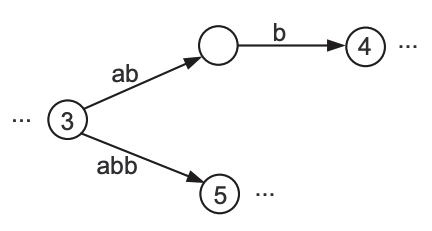
\includegraphics[width=0.78\textwidth]{nd_tg.png}
    \end{center}
    \vspace{-3ex}
\end{blackbox}
    


\begin{blackbox}{Kleene's Theorem}
    \begin{redbox}{Theorem 6}
        \textbf{Theorem.} Any language that can be defined by regular expression, or finite automaton, or transition graph can be defined by all three methods. Proving Kleene's Theorem is done in 3 parts. 
        \begin{itemize}[leftmargin=0.3cm]
            \item \textbf{Part 1:} Every language that can be defined by a finite automaton can also be defined by a transition graph.
            \item \textbf{Part 2:} Every language that can be defined by a transition graph can also be defined by a regular expression.
            \item \textbf{Part 3:} Every language that can be defined by a regular expression can also be defined by a finite automaton. 
        \end{itemize}
        \begin{brownbox}{Proof for Part 3}
            Rules 1-4 show that every regular expression can be converted to a finite automaton.
            \begin{itemize}[leftmargin=0.3cm]
                \item \textbf{Rule 1:} There is an FA that accepts any letter of the alphabet (including $\Lambda$). 
                \item \textbf{Rule 2:} Given $FA_1$ that accepts the language defined by the regular expression \textbf{r}\textsubscript{1} and $FA_2$ that accepts the language defined by \textbf{r}\textsubscript{2}, then there is an FA that accepts the language defined by the regular expression (\textbf{r}\textsubscript{1} + \textbf{r}\textsubscript{2}). 
                \item \textbf{Rule 3:} Given $FA_1$ that accepts the language defined by the regular expression \textbf{r}\textsubscript{1} and $FA_2$ that accepts the language defined by \textbf{r}\textsubscript{2}, then there is an $FA_3$ that accepts the language defined by the regular expression (\textbf{r}\textsubscript{1}\textbf{r}\textsubscript{2}).
                \item \textbf{Rule 4:} If \textbf{r} is a regular expression and $FA_1$ is a finite automaton that accepts exactly the language defined by \textbf{r}, then there is an FA, called $FA_2$, that will accept exactly the language defined by \textbf{r}\textsuperscript{*}
            \end{itemize}
        \end{brownbox}
    \end{redbox}\\[-2ex]
\end{blackbox}
\begin{blackbox}{Nondeterministic Finite Automata}
    \vspace{1ex}
    \textbf{Definition.} A nondeterministic finite automaton (or NFA) is a TGA with a unique start state and with the property that each of its edge labels is a single letter. 
    \begin{bluebox}{Theorem 7}
        \textbf{Theorem. For every NFA, there is some FA that accepts exactly the same language.}
    \end{bluebox}
    \vspace{-2ex}
\end{blackbox}
\begin{blackbox}{Proof 1 of Kleene's Theorem}
        \textbf{Part 1:} This is proved trivially since a finite automaton is a transition graph.\\
        \textbf{Part 2:} Use the following algortithm: 
        \vspace{-1.5ex}
        \begin{enumerate}[leftmargin=0.5cm, noitemsep]
            \item Create a unqiue, unenterable start state and unique, unleaveable final state.
            \item Bypass and eliminate all states that are not start or final states in any order by connecting each incoming edge with each outgoing edge, label the new edge with the concatenation of the labels.
            \item When two states are joined by more than one edge, replace them with a single edge labeled with the union of the labels.
            \item When all that is left is the start and end state, the label of the edge between them is the regular expression that defines the language.
        \end{enumerate}
    \begin{pinkbox}{Proof of Part 3}
        \begin{itemize}[leftmargin=0.3cm, noitemsep]
            \item \textbf{Rule 1:} An FA can easily be created that transitions to the final state on the single letter, then to a garbage state on any other letter.
            \item \textbf{Rule 2:} Algorithm: Start with 2 FA's, $FA_1$ with states $x_1,x_2,\ldots$, $FA_2$ with states $y_1,y_2,\ldots$. Start state will be $z_{start} = x_{start} \text{ or } y_{start}$. To transition to another state, next state will be $z_{new}$ after reading letter $p$ will be $x_{new}$ (next state after reading $p$ on $FA_1$), $y_{new}$ (next state after reading $p$ on $FA_2$). If $x_i$ or $y_1$ are final states, then so is $z_i$.
            \item \textbf{Rule 3:} Algorithm: Create a state $z$ for every state of $FA_1$. For every final state $x_{final}$, add a state $z = x_{final}$ or $y_1$. Then added states $z = x_i$ indicated we are continuing in $FA_1$ or $z = y_i$ indicated we are continuing in $FA_2$. Every final state in $FA_2$ will be a final state.
            \item \textbf{Rule 4:} Algorithm: Create a new start state that will also be a final state so we can accept $\Lambda$. Then, each state $z_i$ in $FA_2$ will correspond to some collection of $x_i$ states in $FA_1$. Set $z_1\pm = x_1-$, then the transition will be based on reading input letters determined by the transition rules in $FA_1$. Once we reach a final state, we have the option to return to the start state $x_1$.
        \end{itemize}
        \begin{bluebox}{Proof 2}
            \textbf{Rule 1:} Design an NFA to accept $a$, $b$, and $\lambda$, use Theorem 7 to construct an FA.\\
            \textbf{Rule 2:} We can construct the union FA $FA_1 + FA_2$ with the following algorithm: First create a unique start state with 2 outgoing $a$-edges and 2 outgoing $b$-edges. Remove minus signs from existing start states, and use theorem 7 to convert to an FA.
        \end{bluebox}
    \end{pinkbox}\\[-2ex]
\end{blackbox}
\begin{blackbox}{Proof of Theorem 7}
    \begin{bluebox}{Proof 1}
        By part 2 of Kleene's theorem, we can convert an NFA into a regular expression. Then, by part 3 of Kleene's theorem, we can convert the regular expression into a finite automaton. Thus we can create an FA from an NFA.
    \end{bluebox}
    \begin{pinkbox}{Proof 2}
        The algorithm for constructing an FA from an NFA is as follows:
        \begin{itemize}[leftmargin=0.3cm]
            \item Each state in the FA is a collection of states from the NFA.
            \item For every state $z$ in FA, the new state that an $a$-edge or $b$-edge takes us to is the collection of possible states that result from being in $x_i$ or $x_j$ and taking that edge and so on.
            \item The start state of the FA is the same as the start state in the NFA.
            \item A state $\phi$ is added since there may be no $a$ edges or $b$-edges from any particular state in the NFA, so an edge to $\phi$ is added.
            \item The state $\phi$ will have an $a,b$-edge to itself.
            \item A state in the FA is a final state if the collection of $x$ states that it represents contains a final state.
        \end{itemize}
    \end{pinkbox}\\[-2ex]
\end{blackbox}
\begin{blackbox}{Mealy and Moore Machine}
    A \textbf{Moore machine} is a collection of 5 things 
    \begin{enumerate}[leftmargin=7pt]
        \item A finite set of states $q_0, q_1, q_2, \ldots$ where $q_0$ is designated as the start state.
        \item An alphabet of letters for forming the input string $\Sigma = \{a,b,c,\ldots\}$
        \item An alphabet of possible output characters $\Gamma = \{0,1,2,\ldots\}$
        \item A transition table that shows for each state and each input letter what state is reached next.
    \end{enumerate}
    A \textbf{Mealy machine} is a collection of 4 things:
    \begin{enumerate}[leftmargin=7pt]
        \item A finite set of states $q_0, q_1, q_2,\ldots$ where $q_0$ is designated as the start state.
        \item An alphabet of letters forming the input string $\Sigma = \{a,b,c,\ldots\}$
        \item An alphabet of possible output characters $\Gamma = \{0,1,2,\ldots\}$
        \item A pictorial representations with states represented by nodes and directed edges indicating transitions.
    \end{enumerate}
\end{blackbox}
\begin{blackbox}{Mealy and Moore Machines}
    The pictorial representation of a Mealy machine has:
    \begin{itemize}[leftmargin=9pt]
        \item Each edge is labeled with a compound symbol of $i/o$, where $i$ is an input letter and $o$ is an output character.
        \item Every state must have exactly one outgoing edge for each possible input letter.
        \item The edge we travel is determined by the input letter $i$. While traveling on the edge, we must print the output character $o$.
    \end{itemize}
    \textbf{Definition.} Given the Mealy machine $Me$ and the Moore machine $Mo$ (which prints at least the start state character $x$), we say that these two are \emph{equivalent} if for every input string from $Mo$ is exactly $x$ concatenated with the output string from $Me$.
    \begin{bluebox}{Theorem 8}
        \textbf{Theorem 8.} If $Mo$ is a Moore machine, then there is a Mealy machine $Me$ that is equivalent to $Mo$.\\[1ex]
        \textit{Proof by Constructive Algorithm:} 
        \begin{itemize}[leftmargin=5pt]
            \item Consider an arbitrary state from $Mo$, say $q_i$, which outputs some character $t$. Suppose it has incoming edges labels with $a,b,c,\ldots$. Relabel the edges with $a/t, b/t, c/t,\ldots$, so we print $t$ on any incoming edge to $q_i$. Repeat this process for all states in $Mo$ and we end up with a Mealy machine $Me$.
        \end{itemize}
    \end{bluebox}
    \begin{redbox}{Theorem 9}
        \textbf{Theorem 9.} For every Mealy machine $Me$, there is a Moore machine $Mo$ that is equivalent to it.\\[1ex]
        \textit{Proof by Constructive Algorithm:}
        \begin{itemize}[leftmargin=5pt]
            \item Consider an arbitrary state from $Me$, $q_i$. If all incoming edges have the same printing character, then we can push the printing character into the state.
            \item If the incoming edges have different printing characters, then we create a new state for each printing character and connect the states with the same input letter.
            \item An edge that was a loop in $Me$ may becomes 2 edges in $Mo$, one that is a loop and one that is not.
            \item If there is a state with no incoming edges, assign it any printing instruction.
            \item If we need to make copies of the start state in $Me$, any of the copies can be the start state in $Mo$.
        \end{itemize}
    \end{redbox}\\[-1ex]
\end{blackbox}
\begin{blackbox}{Regular Languages}
    \textbf{Definition.} A language that can be defined by a regular expression is called a regular language.
\end{blackbox}
\begin{blackbox}{Regular Languages Continued}
    \begin{brownbox}{Theorem 10}
        \textbf{Theorem 10.} If $L_1$ and $L_2$ are regular languages, then $L_1 + L_2$, $L_1L_2$, and $L_1^*$ are also regular languages.\\
        \begin{pinkbox}{Proof 1}
            \begin{itemize}[leftmargin=5pt]
                \item If $L_1$ and $L_2$ are regular languages, then they have regular expressions $\textbf{r}_1$ and $\textbf{r}_2$ that define them. Then $\textbf{r}_1 + \textbf{r}_2$ is a regular expression that defines $L_1 + L_2$.
                \item Similarly, $\textbf{r}_1\textbf{r}_2$ is a regular expression that defines $L_1L_2$, and $L_1^*$ is defined by $\textbf{r}_1^*$.
            \end{itemize}
        \end{pinkbox}
        \begin{redbox}{Proof 2 Using Machines}
            \begin{itemize}[leftmargin=5pt]
                \item Since $L_1$ and $L_2$ are regular languages, there are TGs that accept them $TG_1$ and $TG_2$. Then, suppose $TG_1$ and $TG_2$ have unique start and end states. We can create a new start state that transitions to the start states of $TG_1$ and $TG_2$ on $\Lambda$. From Kleene's theorem, this TG defines $L_1 + L_2$, and has a regular expression that defines it.
                \item Using Kleene's theorem again, we can construct a TG that accepts $L_1L_2$ by having the end state of $TG_1$ transition to the start state of $TG_2$ on $\Lambda$. This TG has a regular expression that defines $L_1L_2$.
                \item Adding 2 edges from the start state to the end state and from the end state to the start state on $\Lambda$ will define $L_1^*$.
            \end{itemize}
            \end{redbox}
    \end{brownbox}
    \textbf{Definition.} If $L$ is a language over the alphabet $\Sigma$, the \emph{complement} of $L'$ is the language of all strings over $\Sigma$ that are not in $L$.\\[1.5ex]
    \begin{bluebox}{Theorem 11}
        \textbf{Theorem 11.} If $L$ is a regular language, then $L'$ is also a regular language.\\[1ex]
        \textit{Proof.} If $L$ is a regular language, then by Kleene's theorem there is an FA that accepts the language $L$.
        \begin{itemize}[leftmargin=5pt]
            \item We can create a new FA that accepts the language $L'$ by reversing each state, final states become non-final states, and vice versa. The start state becomes $\pm$.
            \item Strings that would end on a final state in $L$ now end on a non-final state in $L'$, so it rejects all strings that $L$ accepts. Therefore this machine accepts $L'$.
        \end{itemize}
    \end{bluebox}\\[-2ex]
\end{blackbox}
\begin{blackbox}{Regular Languages: Intersections}
    \begin{redbox}{Theorem 12}
        \textbf{Theorem 12.} If $L_1$ and $L_2$ are regular languages, then $L_1\cap L_2$ is also a regular language.\\[1ex]
        \begin{brownbox}{Proof 1}
            Using DeMorgan's law: $L_1 \cap L_2 = (L_1' + L_2')'$. Theorem 11 tells us $L_1'$ and $L_2'$ are regular, so $L_1' + L_2'$ is also regular, then the complement of that is also regular.
        \end{brownbox}
        \begin{pinkbox}{Proof 2}
            We build a machine $FA_3$ similarly to Kleene's theorem part 3, rule 2, which shows how to build an FA from the union of FA's. We build $FA_3$ the same way but only denote a state final if both corresponding states in $FA_1$ and $FA_2$ are final.
        \end{pinkbox}
    \end{redbox}\\[-2ex]
\end{blackbox}
\begin{blackbox}{Non-regular Languages}
    \textbf{Definition.} A language that cannot be defined by a regula rexpression is called a \emph{non-regular} language.
    \begin{redbox}{Theorem 13}
        \textbf{Theorem 13.} Let $L$ be any regular language that has infinitely many words. Then there exist some three strings $x,y$ and $z$ (where $y$ is not the null string) such that all the strings of the form \\[-0.5ex]
        \[xy^nz, \ n = 1,2,3,\ldots\]
        are words in $L$.\\[1ex]
        \textit{Proof.} Since $L$ is regular, there is a FA that accepts $L$, let $w$ be a word in $L$ that has more letters than there are states in the FA. Then, $w$ must pass through some states multiple times, we can break $w$ into parts:
        \begin{enumerate}[leftmargin=10pt]
            \item Let $x$ denote all the letters of $w$ that lead to the first repeated state. This may be the null string if the circuit starts at the beginning.
            \item Let $y$ denote the substring of $w$ that travels around the circuit back to the repeated state. This must be not the null string since there must be a circuit present in the FA.
            \item Let $z$ be the rest of $w$, starting after $y$ going to the end of $w$.
        \end{enumerate}
        Thus we have $w = xyz$, and we can travel the circuit as many times as we want to have $xy^nz$ be in $L$.
    \end{redbox}\\[-2ex]
\end{blackbox}
\begin{blackbox}{Non-regular Languages Continued}
    \begin{brownbox}{Theorem 14}
        Let $L$ be an infinite language accepted by a finite automaton with $N$ states. Then, for all words $w$ in $L$ that have more than $N$ letters, there are strings $x$, $y$, and $z$, where $y$ is no null and $\length(x) + \length(y)$ does not exceed $N$, such that $w = xyz$ and all strings of the form $xy^nz$ are in $L$.
    \end{brownbox}\\[-1ex]
\end{blackbox}
\begin{blackbox}{Decidability}
    \textbf{Definition.} An effective solution to a problem that has a yes or no answer is called a \emph{decision procedure}. A problem that has a decision procedure is called \emph{decidable}.\\
    Objective is to find methods to determine if the FA $(L_1 \cap L_2') + (L_2 \cap L_1')$ accepts any words. If it accepts any words, then $L_1$ and $L_2$ are not the same.\\
    \begin{pinkbox}{Method 1}
        Convert the FA into a regular expression. Then, any regular expression excepts words by the following algorithm:
        \begin{itemize}[leftmargin=5pt]
            \item Remove all stars from the regular expression.
            \item For each $+$, remove the right half and take the left.
            \item Remove parentheses and have just concatenations of $a$'s and $b$'s which forms a word.
        \end{itemize}
        If the FA $(L_1 \cap L_2') + (L_2 \cap L_1')$ produces a regular expression, then by method 1 it must define some words so $L_1$ is not the same as $L_2$.
    \end{pinkbox}
    \begin{redbox}{Method 2}
        Examine the FA $(L_1 \cap L_2') + (L_2 \cap L_1')$ and see if there is a path from $-$ to $+$. If there is a path, then the machine accepts some words. Procedure for large FAs: 
        \begin{enumerate}[leftmargin=5pt]
            \item Paint the start state blue.
            \item For every blue state, follow each outgoing edge and paint the destination state blue. Remove that edge.
            \item Repeat step 2 until no new state is painted blue. 
            \item If any of the final states are blue, then the machine accepts some words. If no final states are blue, then the machine does not accept any words.
        \end{enumerate}
    \end{redbox}
    \begin{bluebox}{Theorem 17}
        \textbf{Theorem 17.} Let $F$ be an FA with $N$ states. Then, if $F$ accepts any words, it accepts some words with fewer than $N$ letters.
    \end{bluebox}\\[-2ex]
\end{blackbox}
\begin{blackbox}{Decidability Continued}
    \begin{bluebox}{Thereom 17 Proof}
        \textit{Proof.} If $F$ accepts some word $w$, then $w$ generates a path from $-$ to $+$. If $\length(w) < N$, then we are done. 
        \begin{itemize}[leftmargin=5pt]
            \item If $\length(w) \geq N$, then the path must have a circuit from $-$ to state $m$ then back to state $m$ and to $+$.
            \item Then there is a path from $-$ to state $m$ and to $+$ without traveling through the circuit that would be shorter, and can visit each state at most once. Thus it has at most $N-1$ edges and will accept a word of at most $N-1$ letters.
        \end{itemize}
    \end{bluebox}
    \begin{brownbox}{Method 3}
        Test al wrods with fewer than $N$ letters by running them through the FA. If the FA accepts none of them, then it accepts no words (using Theorem 17).        
    \end{brownbox}
    Theorem 18 summarizes the 3 previous results: \\[1ex]
    \textbf{Theorem 18.} There is an effective procedure to decide whether:
    \begin{enumerate}[leftmargin=15pt]
        \item A given FA accepts any words.
        \item Two FAs are equivalent.
        \item Two regular expressions are equivalent.
    \end{enumerate}

    \textbf{Finiteness.} A regular expression defines a finite language if and only if it does not contain the Kleene star. 
    
    \begin{redbox}{Theorem 19}
        \textbf{Theorem 19.} Let $F$ be a FA with $N$ states. Then, $F$ accepts infinitely many words if and only if it accepts some word $w$ such that \\[-2ex]
        \[N \leq \length(w) \leq 2N\]
    \end{redbox}
    \begin{pinkbox}{Theorem 20}
        There is an effective procedure to decide whether a given FA accepts an finite or an infinite language.\\[1ex]
        \textit{Proof.} Suppose the FA has $N$ states over an alphabet with $m$ letters. Then there are $m^{N}$ strings of length $N$, and $m^{N+1}$ strings of length $N+1$, and so on. So there are a finite number of strings of lengths between $N$ and $2N$, \\[-1ex]
        \[m^N + m^{N+1} + m^{N+2} + \cdots + m^{2N-1}\]
        We can test each of these strings and if any are accepted, the language is infinite.
    \end{pinkbox}\\[-2ex]
\end{blackbox}
\begin{blackbox}{Context Free Grammars}
    \textbf{Definition.} A \textbf{context-free gammar} (CFG) is a collection of 3 things:
    \begin{enumerate}[leftmargin=7pt]
        \item An alphabet $\Sigma$ of letters called \textbf{terminals} from which we make strings that will be words of a language.
        \item A set of symbols called \textbf{nonterminals}, one of which is the symbol $S$ which is the start symbol.
        \item A finite set of \textbf{productions} of the form \\[-4ex]
        \[\text{Nonterminal} \rightarrow \text{terminals and/or nonterminals}\]
    \end{enumerate}
    \vspace{-2ex}
    \textbf{Definition.} The \emph{language generated by a CFG} is the set of all strings of terminals that can be produced from the start symbol $S$ using the productions as substitutions. A language generated by a CFG is called a \emph{context-free language} (CFL).
    \begin{bluebox}{Trees}
        Start with the symbol $S$, every time we use a production to replace a nonterminal, draw downward lines from the nonterminal to each caracter in the string.\\[-6ex]
        \begin{center}
            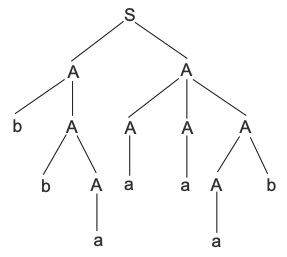
\includegraphics[width=0.6\textwidth]{cfg_tree.png}
        \end{center}
        Reading the leaves from left to right gives the string generated by the CFG.
    \end{bluebox}
    \begin{redbox}{Lukasiewicz Notation}
        Walk around the tree and write down each symbol once that we visit, traverse down the left side of the tree first.\\
        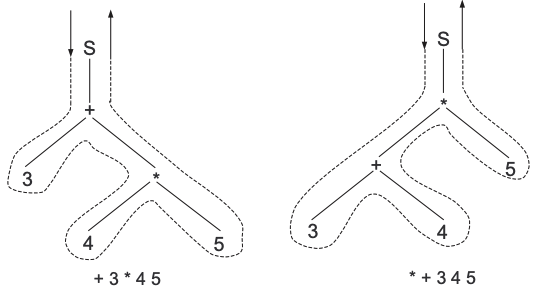
\includegraphics[width=1\textwidth]{ln.png}
        Then the strings are in prefix notation, which we say is \emph{unambiguous}.
    \end{redbox}\\[-2ex]
\end{blackbox}
\begin{blackbox}{Ambiguity}
    \textbf{Definition.} A CFG is called \textbf{ambiguous} if for at least one word in the language that it generates, there are 2 possible derivation trees.\\
    \textbf{Definition.} For a given CFG, we define a tree with the start symbol $S$ as its root and whose nodes are working strings of terminals and nonterminals. The descendants of each node are all possible results applying every production. This tree is called the \textbf{total language tree}.\\
    \textbf{Example:} Consider the CFG: 
    \begin{align*}
        S &\rightarrow aa | bX | aXX\\
        X &\rightarrow ab|b
    \end{align*}
    \begin{center}
        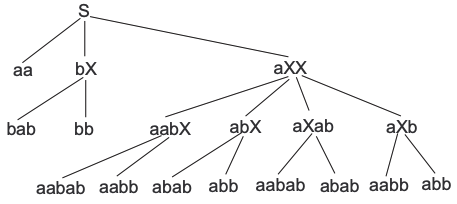
\includegraphics[width=0.9\textwidth]{total_tree.png}
    \end{center}
\end{blackbox}
\begin{blackbox}{Grammatical Format}
    \textbf{Definition.} For a given CFG, a \textbf{semi-word} is a string of terminals (maybe none) concatenated wih exactly one nonterminal on the right.
    \begin{bluebox}{Theorem 21}
        \textbf{Theorem 21.} Given any FA, there is a CFG that generates exactly the language accepted by the FA. In other words, all regular languages are context-free languages.\\[1ex]
        \textit{Proof.} Constructive Algorithm
        \begin{itemize}[leftmargin=5pt]
            \item Step 1: Nonterminals in the CFG will be states in the FA, and $S$ will be the start state.
            \item Step 2: Every edge will be a production, so $X \rightarrow aY$ would be a production if there is an edge from $X$ to $Y$ on $a$.
            \item For every final state $F$, create the production $F \rightarrow \boldsymbol{\Lambda}$.
        \end{itemize}
    \end{bluebox}
    \begin{redbox}{Theorem 22}
        \textbf{Theorem 22.} If every production is of the form 
        \[\text{Nonterminal} \rightarrow \text{semi-word or word} \]
        Where word may be $\boldsymbol{\Lambda}$, then the language generated by this CFG is regular.
    \end{redbox}
\end{blackbox}
\begin{blackbox}{Grammatical Format Continued}
    \begin{redbox}{Proof of Theorem 22}
        Consider a general CFG with productions $N_1 \rightarrow w_1N2$, $N_2 \rightarrow w_2N_3,\ldots, N_i \rightarrow w_i$, so $wN$'s are semi-words. We want to construct a TG that accepts the same language so that by Kleene's theorem it is regular.
        \begin{itemize}[leftmargin=5pt]
            \item Let $N_1 = S$, and for every production $N_x \rightarrow w_yN_z$ draw a directed edge between $N_x$ to $N_z$ labeled with $w_y$. If $N_x = N_z$, then we have a loop.
            \item For every production of the form $N_p \rightarrow w_q$, then we draw an edge from the state $N_p$ to the $+$ state and label it $w_q$.
            \item Any path from $-$ to $+$ is a word in the language of the TG and is also a sequence of productions in the CFG, and on the otherhand any derivation in this CFG
            \[S \Rightarrow w_iN_x \Rightarrow w_iw_j N_y \Rightarrow \cdots \Rightarrow w_iw_j\cdots w_q\]
            corresponds to a path in the TG.
        \end{itemize} 
        Therefore the language of this TG is the same as that of the CFG and the CFG is regular.
    \end{redbox}
    \textbf{Definition.} A CFG is called a \textbf{regular grammar} if each of its productions is as described in Theorem 22.\\[1ex]
    \textbf{Definition.} In a given CFG, we call a nonterminal $N$ \textbf{nullable} if there is a derivation of the form $N \Rightarrow \Lambda$.\\
    \begin{brownbox}{Theorem 23}
        \textbf{Theorem 23.} If $L$ is a context-free language generated by a CFG that includes $\boldsymbol{\Lambda}$-productions, then there is CFG that generates $L$ without $\boldsymbol{\Lambda}$\\[1ex]
        \textit{Proof.} Given a CFG with $\Lambda$-productions, we can convert it using the algorithm: 
        \begin{enumerate}[leftmargin=7pt]
            \item Delete all $\Lambda$-productions.
            \item For every production $N \rightarrow \text{nullable string}$, we replace it with a new string that can be formed by deleting all possible subsets of nullable nonterminals.
        \end{enumerate}
    \end{brownbox}
    \textbf{Definition.} A production of the form \\[-1.5ex]
    \[\text{Nonterminal} \rightarrow \text{One Nonterminal}\]
    is callued a \textbf{unit production}.
    \begin{pinkbox}{Theorem 24}
        \textbf{Theorem 27.} If there is a CFG for the language $L$ that no $\boldsymbol{\Lambda}$-productions, then there is also a CFG for $L$ with no null productions or unit productions.
    \end{pinkbox}\\[-2ex]
\end{blackbox}
\begin{blackbox}{Grammatical Format Continued}
    \begin{pinkbox}{Proof of Theorem 24}
        \textit{Proof. Constructive Algorithm.} For every pair of nonterminals $A$ and $B$, if the CFG has a unit production $A \rightarrow B$, or a chain \\[-2ex]
        \[A \rightarrow X_1 \rightarrow X_2 \rightarrow \cdots \rightarrow B\]
        where $X_1,\ldots,$ are nonterminals, create new productions as follows: If the non-unit productions from $B$ are \\[-4ex]
        \[B \rightarrow s_1|s_2|\cdots\] 
        where $s_1,s_2,\ldots$ are strings, we create the productions \\[-4ex]
        \[A \rightarrow s_1|s_2| \cdots\]
    \end{pinkbox}
        \begin{brownbox}{Chomsky Normal Form (Theorem 25)}
            A method of seperating terminals from nonterminals in productions.\\
            \textbf{Theorem 25.} If $L$ is a language generated by some CFG, then there is another CFG that generates all the non-$\boldsymbol{\Lambda}$ words of $L$, all of whose products are of the form\\[-1ex]
            \[\text{Nonterminal} \rightarrow \text{String of Nonterminals}\]
            or\\[-1.25ex]
            \[\text{Nonterminal} \rightarrow \text{One Terminal}\]
            \textit{Proof. Constructive Algorithm.} 
            \begin{itemize}[leftmargin=5pt]
                \item Suppose the nonterminals in a CFG are $S, X_1, X_2,\ldots$ and the terminals are $a$ and $b$. Then create 2 new nonterminals $A$ and $B$ with the productions $A \rightarrow a$ and $B \rightarrow b$. 
                \item Then for each of the existing productions, replace any terminals $a$ and $b$ with the nonterminals $A$ and $B$.
                \item Then each production will be a string of nonterminals, along with the 2 productions which are of the form $\text{Nonterminal} \rightarrow \text{One Terminal}$.
            \end{itemize}
        \end{brownbox}
        \textbf{Definition.} If a CFG has only productions of the form \\[-3ex]
        \[\text{Nonterminal} \rightarrow \text{String of Exactly 2 Nonterminals}\]
        or of the form \\[-3ex]
        \[\text{Nonterminal} \rightarrow \text{One Terminal}\]
        then it is said to be in \textbf{Chomsky Normal Form} (CNF).
        \begin{bluebox}{Theorem 26}
            For any context-free language $L$, the non-$\boldsymbol{\Lambda}$ words of $L$ can be generated by a grammar in which all productions are in CNF.
        \end{bluebox}\\[-2ex]
\end{blackbox}
\begin{blackbox}{Grammatical Format Continued}
    \begin{bluebox}{Proof of Theorem 26}
        \textit{Proof. Constructive Algorithm.} From theorem 23 and 24, we know that there is a CFG for $L$ (not including $\boldsymbol{\Lambda}$) that has no $\boldsymbol{\Lambda}$-productions or unit productions. Then we can make the CFG fit the form specified in Theorem 25.
        \begin{itemize}[leftmargin=5pt]
            \item For the productions 
            \[\text{Nonterminal} \rightarrow \text{One Terminal}\]
            we leave them alone.
            For the other productions of the form \\[-1ex]
            \[\text{Nonterminal} \rightarrow \text{String of Nonterminals}\]
            we introduce new nonterminals $R_1,R_2,\ldots$ so that each string of nonterminals is of length 2. For example, $S \rightarrow X_1X_2X_3X_4$ becomes\\[-1ex]
            \[S \rightarrow X_1R_1, R_1 \rightarrow X_2R_2, R_2 \rightarrow X_3X_4\]
            So all productions which are a string of nonterminals become a sequence of productions with exactly 2 nonterminals.
        \end{itemize}
    \end{bluebox}
    \textbf{Definition.} The \textbf{leftmost nonterminal} in a woroking string is the first nonterminal that we encounter when we scan the string from left to right.\\
    \textbf{Example.} In $abNbaXYa$, leftmost nonterminal is $N$. \\
    \textbf{Definition.} IF a word $w$ is generated by a CFG such that at each step in the derivation, a production is applied to the leftmost non terminal in the working tree, then this derivation is called a \textbf{leftmost derivation}.\\
    \begin{redbox}{Theorem 27}
        \textbf{Theorem 27.} Any word that can be generated by a given CFG by some derivation also has a leftmost derivation.
    \end{redbox}

\end{blackbox}
\begin{blackbox}{Pushdown Automata}
    \textbf{Definition.} The \textbf{input tape} is part of the machine where the input is placed. It is divided into cells containing characters and is terminiated with $\Delta$.\\[1ex]
    \textbf{Symbols.} In a PDA, start is denoted by a node with "START", dead-end final states are denoted "ACCEPT", and non-final dead-end states are denoted "REJECT". "READ" states are diamond-shaped boxes with branches for each letter and $\Delta$ for end of string.\\[1ex]
    \textbf{Pushdown Stack:} A place where input letters can be stored and retrieved. Has 2 operations, "PUSH" which adds a new letter to the top of the stack, and "POP" which takes a letter out from the top.
\end{blackbox}
\begin{blackbox}{Pushdown Automata Continued}
    Branching is only allowed on POP and READ states where there can be different paths depending on the letter read.\\
    \textbf{Example.} This PDA accepts the language $\{a^nb^n\}$
    \begin{center}
        
        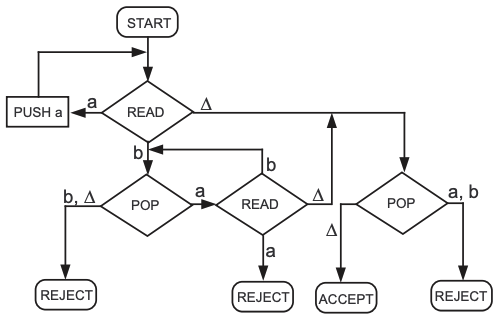
\includegraphics[width=0.69\textwidth]{pda.png}
    \end{center}
        \begin{bluebox}{Deterministic vs Nondeterministic PDA}
        A \textbf{deterministic PDA} is one for which every input string has a unique path through the machine.\\
        A \textbf{nondeterministic PDA} is one for which at certain times we may have to choose among possible paths through the machine.
        \begin{itemize}[leftmargin=5pt]
            \item An input string is accepted by a nondeterministic PDA if \emph{some} set of choices lead us to an ACCEPT state.
            \item If \emph{all possible} paths end in a REJECT state, then the string is rejected.
        \end{itemize}
        \begin{multicols*}{2}
            Note that nondeterminism does increase the power of the PDA to accept new languages unlike with FAs.
            \begin{center}
                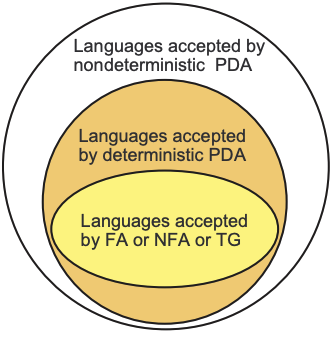
\includegraphics[width=0.49\textwidth]{circles.png}
            \end{center}
        \end{multicols*}
    \end{bluebox}
    \textbf{Definition.} A \textbf{pushdown automata} (PDA) is a collection of 8 things:
    \begin{enumerate}[leftmargin=10pt]
        \item An alphabet $\Sigma$ of input letters.
        \item An inpute TAPE.
        \item An alphabet $\Gamma$ of STACK characters.
        \item A pushdown STACK.
        \item One START state with only out-edges.
        \item Halt states, ACCEPT and REJECT (no out-edges).
        \item Finitely many non-branching PUSH states.
        \item Finitely many branching states, READ and POP.
    \end{enumerate}
\end{blackbox}
\begin{blackbox}{Pushdown Automata Continued}
    \begin{redbox}{Theorem 28}
        \textbf{Theorem 28.} For every regular language $L$, there is some PDA that accepts it.\\[1ex]
        \textit{Proof.} Since $L$ is regular, there is an FA that accepts it. We can convert this FA into a PDA directly by using START, READ, ACCEPT, and REJECT states.
    \end{redbox}
    \begin{brownbox}{Theorem 29}
        \textbf{Theorem 29.} Given any PDA, there is another PDA that accepts exactly the same language with the additional property that whenever a path leads to ACCEPT, the STACK and the TAPE contain only blanks.\\[1ex]
        \textit{Proof. Constructive Algorithm.} Each time we see an ACCEPT we replace it with
        \begin{center}
            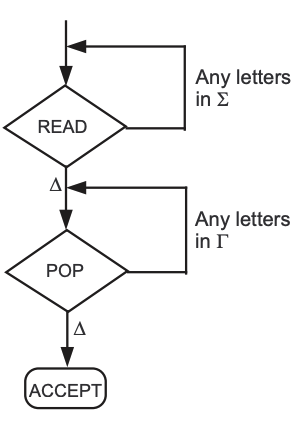
\includegraphics[width=0.5\textwidth]{t29.png}
        \end{center}
    \end{brownbox}\\[-2ex]
\end{blackbox}
\begin{blackbox}{CFG = PDA}
    \textbf{Theorem 30.} Given a CFG that generates the language $L$, there is a PDA that accepts exactly $L$.\\[1ex]
    \textbf{Theorem 31.} Given a PDA that accepts the language $L$, there exists a CFG that generates exactly $L$.\\[1ex]
    \textit{Proof. Constructive Algorithm.} Given a CFG in CNF as\\[-0.5ex]
    \[X_1 \rightarrow X_2X_3,\ X_1 \rightarrow X_3X_4,\ X_2 \rightarrow X_2X_2, \cdots\]
    \[X_3 \rightarrow a,\ X_4 \rightarrow a,\ X_5 \rightarrow b, \ldots\]
    We construct the PDA as follows, start with:
    \begin{center}
        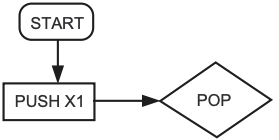
\includegraphics[width=0.5\textwidth]{th30_1.png}
    \end{center}
\end{blackbox}
\begin{blackbox}{Proof of CFG = PDA Continued}
    \begin{multicols*}{2}
        \begin{minipage}{0.45\textwidth}
        For each production of the form $X_i \rightarrow X_jX_k$, we include this circuit from the POP state back to itself
        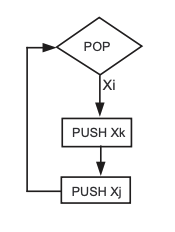
\includegraphics[width=1\textwidth]{th30_2.png}
    \end{minipage}
    \begin{minipage}{0.45\textwidth}
        For each production of the form $X_i \rightarrow b$, we include the circuit.

        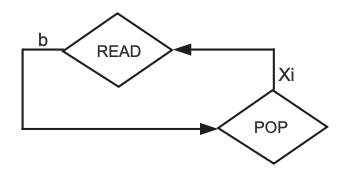
\includegraphics[width=1\textwidth]{th30_3.png}
        
        When the STACK is empty, which means we converted our last nonterminal to a terminal and the terminals have matched the INPUT TAPE, add this path:
    \end{minipage}
    \end{multicols*}
    \begin{center}
        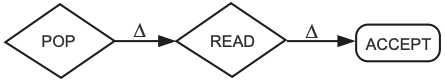
\includegraphics[width=0.9\textwidth]{th30_4.png}
    \end{center}
\begin{itemize}
    \item At the beginning we assumed that the CFG was in CNF, but there are CFLs that cannot be put into CNF because they include the word $\boldsymbol{\Lambda}$.
    \item In this case, convert all productions into CNF and construct the PDA as described above, then add this circuit at the POP to kill the nonterminal S without replacing it with anything.
\end{itemize}
    \begin{center}
        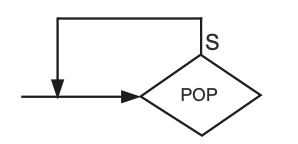
\includegraphics[width=0.6\textwidth]{th30_5.png}
    \end{center}
    Proof of Theorem 31 is not included, together Theorems 30 and 31 prove CFG = PDA.
\end{blackbox}
\begin{blackbox}{Context-Free Languages}
    \begin{pinkbox}{Theorem 36}
        Let $L_1$ and $L_2$ be context-free languages. Then their union $L_1 + L_2$ is also a context free language.\\
        \textit{Proof. Constructive Algorithm.} Let the CFG for $L_1$ have start symbol $S_1$, and $L_2$ has start symbol $S_2$.
        \begin{itemize}[leftmargin=5pt]
            \item Define new start symbol $S \rightarrow S_1 | S_2$. 
            \item Then for if we begin with $S \Rightarrow S_1$, all words derived will belong to $L_1$. Similarly for $S_2$.
        \end{itemize}
    \end{pinkbox}\\[-2ex]
\end{blackbox}
\begin{blackbox}{Context-Free Languages Continued}
    \begin{pinkbox}{Proof 2 of Theorem 36 Using Machines}
        From Theorem 30 we know that there is a PDA that accepts $L_1$ and $L_2$, we can then construct a third PDA which has replaces the 2 START states with 1 new START state with 2 outgoing edges, one to the PDA corresponding to $L_1$ and the other to the PDA corresponding to $L_2$.
    \end{pinkbox}
    \begin{brownbox}{Theorem 37}
       \textbf{Theorem 37.} Let $L_1$ and $L_2$ be context-free languages. Then, $L_1L_2$ is also a context-free language.\\[1ex]
        \textit{Proof. Constructive Algorithm.} 
        \begin{itemize}[leftmargin=7pt]
            \item Let $CFG_1$ be the context-free grammar for $L_1$ having start state $S_1$ and nonterminals $A_1,B_1,C_1,\ldots$.
            \item Let $CFG_2$ be the context-free grammar for $L_2$ having start state $S_2$ and nonterminals $A_2,B_2,C_2,\ldots$.
            \item Then, we use all the nonterminals and productions from $CFG_1$ and $CFG_2$, adding a new start symbol $S$ and the production $S \rightarrow S_1S_2$.
        \end{itemize}
    \end{brownbox}
    \begin{redbox}{Theorem 38}
        \textbf{Theorem 38.} If $L$ is a context-free language, then $L^*$ is also a context-free language.\\[1ex]
        \textit{Proof.} We start with a CFG for the language $L$ with the start state $S_1$. Then, using all the nonterminals and productions of the CFG for $L$, we add a new start symbol $S$ and production $S \rightarrow S_1S|\boldsymbol{\Lambda}$. Using this gives us the derivation \\[-2.75ex]
        \[S \Rightarrow S_1S \Rightarrow S_1S_1 \Rightarrow \cdots \Rightarrow S_1S_1S_1\cdots S_1\] 
        So in general we can derive $S \Rightarrow S_1^n$, which allows us to generate any word in $L^*$.
    \end{redbox}
    \begin{bluebox}{Theorem 39}
        \textbf{Theorem 39.} The intersection of two context-free languages may or may not be context-free.\\[1ex]
        \textit{Proof.} We know from Theorem 21 that all regular languages are context-free, when $L_1$ and $L_2$ are regular (thus context-free), in this case the intersection 
        will be regular and thus context free.\\[1ex]
        Counter example: $L_1 = \{a^nb^na^m\}$, and $L_2 = \{a^nb^ma^m\}$ we can show these are both context-free. Then,\\[-3ex]
         \[L_3 = L_1 \cap L_2 = \{a^nb^na^n\}\]
         This language is not context-free.
    \end{bluebox}\\[-2ex]
\end{blackbox}
\begin{blackbox}{Context-Free Languages Continued}
    \begin{redbox}{Theorem 40.}
        \textbf{Theorem 40.} The complement of a context-free language may or may not be context-free.\\[1ex]
        \textit{Proof.} We can see again that if $L_1$ were a regular language (and thus context-free), then it would be closed under complementation and will remain context-free. However, in general, for a contradiction:
        \begin{itemize}[leftmargin=7pt]
            \item Suppose the complement of every CFL is context-free, let $L_1$ and $L_2$ be CFL's.
            \item Then $L_1' + L_2'$ is context-free by Theorem 36, and $(L_1'+L_2')'$ is context-free by assumption.
            \item But $(L_1'+L_2')' = L_1 \cap L_2$ which contradicts Theorem 39 since $L_1$ and $L_2$ are any CFL's.  
        \end{itemize}
    \end{redbox}
    \begin{brownbox}{Theorem 41}
        \textbf{Theorem 41.} The intersection of a context-free language and a regular language is always context-free.\\[1ex]
        \textit{Proof. Constructive Algorithm.} We have a PDA for the CFL and an FA for the regular language. Then, we can assume the PDA terminates with a blank STACK and TAPE (using Theorem 29). 
        \begin{itemize}[leftmargin=7pt]
            \item Label each state of the PDA with the name of the particular $x$-state in the FA that the input string would be in if it were being processed on the FA.
            \item We label the START state of the PDA with $x_1$ which is the start state of the FA.
            \item If from START we go to PUSH or POP, then we stay in $x_1$ since we have not read any input yet.
            \item If we enter a READ state, we stay in FA, but when we leave the READ state by either the $a$ or $b$ edge, it will correspond to entering a new state in the FA.
            \item The PDA may be nondeterministic, so there may be several $a$-edges leaving a READ state, and we must label each of the states it takes us to with the $x$-state from the FA that an $a$-edge would take us.
            \item Special case: If in the FA, an a-edge takes us to $x_3$, and a $b$-edge takes us to $x_8$; but in the PDA both the $a$-edge and the $b$-edge takes us to the same state, we must make 2 copies of the state in the PDA state with identical set of exiting edges;  One copy entered by the $a$-edge and labeled $x_3$, the other entered by the $b$-edge and labeled $x_8$.
        \end{itemize}
    \end{brownbox}\\[-2ex]
\end{blackbox}
\begin{blackbox}{Proof of Theorem 41 Continued}
    \begin{itemize}[leftmargin=7pt]
        \item If we revist a state in the PDA that is already labeled, we may need to create another copy of that state.
        \item If the processing of an input string ends in an ACCEPT state that is labeled with $x_m$ where $x_m$ is not a final state in the FA, then that input string would not be accepted.
        \item All ACCEPT states labaled with non-final $x$-states must be REJECT states.
    \end{itemize}
\end{blackbox}



\end{multicols*}
\end{document}
    
